\documentclass[aspectratio=169]{beamer}

%% -------------------------------------------------------------------
%% Theme Configuration
%% -------------------------------------------------------------------
\usetheme[]{iee}

%% -------------------------------------------------------------------
%% Packages
%% -------------------------------------------------------------------
\usepackage{fontawesome5}
\usepackage{pgfplots}
\usepackage{pgf-pie}
\pgfplotsset{compat=1.18} % or your current pgfplots version
\usepackage[table]{xcolor}
\usepackage{csquotes} % Recommended with babel + biblatex
\usepackage{tabularray}
\UseTblrLibrary{booktabs} % Optional, for better lines in tables
\UseTblrLibrary{siunitx}


\usepackage[
  backend      = biber,
  style        = ieee,
  minnames     = 1,
  maxcitenames = 2,
  maxbibnames  = 3,
]{biblatex}
\addbibresource{references.bib}

\DefineBibliographyStrings{german}{
  andothers = {et al.}
}

%% -------------------------------------------------------------------
%% Metadata
%% -------------------------------------------------------------------
% Select language
\usepackage[english]{babel}
% \usepackage[ngerman]{babel}

\title[Short Title]{IEE Template}
\subtitle{for \LaTeX~Presentations}

\author{Robert Gaugl}
\newcommand{\academictitlesauthor}{Ass.Prof. Dipl.-Ing. Dr.techn.}
\newcommand{\coauthors}{}

\date{Presentation Date}

\newcommand{\university}{Graz University of Technology}
\institute{Institute of Electricity Economics and Energy Innovation}
\newcommand{\street}{Inffeldgasse 18}
\newcommand{\postalcode}{8010}
\newcommand{\city}{Graz}
\newcommand{\country}{Austria}

\newcommand{\phone}{+43 316 873 7904}
\newcommand{\mailauthor}{robert.gaugl@tugraz.at}
\newcommand{\urlinstitute}{iee.tugraz.at} % Without https://

\newcommand{\urlinstagram}{instagram.com/iee.tugraz} % Without https://
\newcommand{\urllinkedin}{instagram.com/iee.tugraz} % Without https://

% \logobar{Supported by: 
\includegraphics[height=1cm]{beamerthemeiee/Logo_IEE_DE.png}} % titlepage sponsors or funding agency

%% -------------------------------------------------------------------
%% Options
%% -------------------------------------------------------------------
% Set globally whether paused content appears transparent or is completely hidden.
% This setting can also be changed locally within individual slides to mix styles.
\setbeamercovered{transparent} % options: transparent or invisible

% Activate navigation symbols in the lower left corner
% \activatenavigationbuttonstrue


% Change how numbers appear when using \SI{}{}
\germanenglish{%
    \sisetup{
        output-decimal-marker = {,},  % use comma as decimal separator
        group-separator = {.},        % use dot as thousand separator
        group-minimum-digits = 4,     % format large numbers
        group-digits=integer,
        detect-mode = true,
        detect-family = false,
    }         
    }{
    \sisetup{
        output-decimal-marker = {.},  % use comma as decimal separator
        group-separator = {~},        % use space as thousand separator
        group-minimum-digits = 4,     % optional: format large numbers
        group-digits=integer,
        detect-mode = true,
        detect-family = false,
    }
}
\DeclareSIUnit \watthour { Wh } %apparent power 

%% -------------------------------------------------------------------
%% Document
%% -------------------------------------------------------------------
\begin{document}

%% -------------------------------------------------------------------
%% Title Slide
\begin{frame}[plain]
    \maketitleslide
\end{frame}


%% -------------------------------------------------------------------
%% Section: Understand the Template for a Consistent Layout
\section{Understand the \textbf{Template} for a Consistent Layout}

\begin{frame}
    \agenda
    % Customized agenda:
    % \agenda[sections=all or currentsection][title][subtitle][picture][picture source]
\end{frame}


\begin{frame}{Template}
    \framesubtitle{Footnote and Language}

    % Insert a Faded picture (ALWAYS FIRST THING IN A FRAME)
    \insertfadedpicture{15.98cm}{figures/iee_besprechung.png}{Source: Institute of Electricity Economics and Energy Innovation/TU Graz}
    
    \begin{minipage}{0.8\textwidth}  % 80% of the slide width
        \begin{itemize}
            \item To \textcolor{yellow}{\textbf{change}} text/name in \textcolor{yellow}{\textbf{Footnote}} and \textcolor{yellow}{\textbf{Date on Title Slide}}: 
            \vspace{-0.5\topsep}
            \begin{itemize}
                \item The presentation.tex file contains a section at the top labeled Metadata
                \item Modifying the author, date, or institute in this section will automatically update the footnote and date displayed in the presentation
            \end{itemize}
    
            \item Footnote Text
            \vspace{-0.5\topsep}
            \begin{itemize}
                \item The \textcolor{green}{\textbf{default footnote}} text displays the \textcolor{green}{\textbf{institute's name}}
                \item If you want to include your \textcolor{green}{\textbf{lecture title}}, \textcolor{green}{\textbf{presentation topic}}, or other context-specific information in the \textcolor{green}{\textbf{footnote}}, simply enter it in the \textcolor{green}{\textbf{institute field}} within the metadata section
            \end{itemize}
            
            \item Language
            \vspace{-0.5\topsep}
            \begin{itemize}
                \item Ensure that the \textcolor{iee}{\textbf{language}} used throughout the presentation \textcolor{iee}{\textbf{remains consistent}}
                \item For presentations in \textcolor{iee}{\textbf{German}}, set \textcolor{iee}{\textbf{language pack to german}} in the metadata section.
                \item The \textcolor{iee}{\textbf{footnote text}} must \textcolor{iee}{\textbf{match}} the \textcolor{iee}{\textbf{language}} of the presentation
            \end{itemize}
        \end{itemize}
    \end{minipage}
\end{frame}


\begin{frame}{Color palette}
    \framesubtitle{Make use of the the Defined Colors}
    \label{frame:color_palette}
    
    \vspace{1cm}
    \begin{columns}[t]
        \column{.25\textwidth}
            \begin{beamercolorbox}[center,colsep*=4pt]{white}\textbf{Light Shades}\strut\end{beamercolorbox}
            \begin{beamercolorbox}[center,colsep*=4pt]{white}\strut\end{beamercolorbox}
            \begin{beamercolorbox}[center,colsep*=4pt]{greyLight}greenLight\strut\end{beamercolorbox}
            \begin{beamercolorbox}[center,colsep*=4pt]{blueLight}blueLight\strut\end{beamercolorbox}
            \begin{beamercolorbox}[center,colsep*=4pt]{ieeLight}ieeLight\strut\end{beamercolorbox}
            \begin{beamercolorbox}[center,colsep*=4pt]{redLight}redLight\strut\end{beamercolorbox}
            \begin{beamercolorbox}[center,colsep*=4pt]{turquoiseLight}turquoiseLight\strut\end{beamercolorbox}
            \begin{beamercolorbox}[center,colsep*=4pt]{greenLight}greenLight\strut\end{beamercolorbox}
            \begin{beamercolorbox}[center,colsep*=4pt]{yellowLight}yellowLight\strut\end{beamercolorbox}
        \column{.25\textwidth}
            \begin{beamercolorbox}[center,colsep*=4pt]{white}\textbf{Standard}\strut\end{beamercolorbox}
            \begin{beamercolorbox}[center,colsep*=4pt]{white}\strut\end{beamercolorbox}
            \begin{beamercolorbox}[center,colsep*=4pt]{grey}grey\strut\end{beamercolorbox}
            \begin{beamercolorbox}[center,colsep*=4pt]{blue}blue\strut\end{beamercolorbox}
            \begin{beamercolorbox}[center,colsep*=4pt]{iee}iee\strut\end{beamercolorbox}
            \begin{beamercolorbox}[center,colsep*=4pt]{red}red\strut\end{beamercolorbox}
            \begin{beamercolorbox}[center,colsep*=4pt]{turquoise}turquoise\strut\end{beamercolorbox}
            \begin{beamercolorbox}[center,colsep*=4pt]{green}green\strut\end{beamercolorbox}
            \begin{beamercolorbox}[center,colsep*=4pt]{yellow}yellow\strut\end{beamercolorbox}
        \column{.25\textwidth}
            \begin{beamercolorbox}[center,colsep*=4pt]{white}\textbf{Dark Shades}\strut\end{beamercolorbox}
            \begin{beamercolorbox}[center,colsep*=4pt]{white}\strut\end{beamercolorbox}
            \begin{beamercolorbox}[center,colsep*=4pt]{greyDark}greyDark\strut\end{beamercolorbox}
            \begin{beamercolorbox}[center,colsep*=4pt]{blueDark}blueDark\strut\end{beamercolorbox}
            \begin{beamercolorbox}[center,colsep*=4pt]{ieeDark}ieeDark\strut\end{beamercolorbox}
            \begin{beamercolorbox}[center,colsep*=4pt]
            {redDark}redDark\strut\end{beamercolorbox}
            \begin{beamercolorbox}[center,colsep*=4pt]{turquoiseDark}turquoiseDark\strut\end{beamercolorbox}
            \begin{beamercolorbox}[center,colsep*=4pt]{greenDark}greenDark\strut\end{beamercolorbox}
            \begin{beamercolorbox}[center,colsep*=4pt]{yellowDark}yellowDark\strut\end{beamercolorbox}
    \end{columns}
\end{frame}


%% -------------------------------------------------------------------
%% Leverage Boxes to Organize Content
\section{Leverage \textbf{Boxes} to Organize Content}

\begin{frame}
    \agenda     
    % Customized agenda:     
    % \agenda[sections=all or currentsection][title][subtitle][picture][picture source]
\end{frame}


\begin{frame}{Boxes}
    \framesubtitle{Organize your Content}

    \begin{coloredblock}[yellow]
        \begin{itemize}
            \item \textbf{Instead} of using \textbf{lists} or \textbf{enumerations}, consider \textbf{organizing} your \textbf{content} into \textbf{distinct groups} for better structure
            \item \textbf{Boxes} are an \textbf{excellent tool} to enhance \textbf{visual clarity} and emphasize group distinctions
        \end{itemize}
    \end{coloredblock}

   % Bottom blocks (side-by-side)
    \begin{columns}
        \begin{column}{0.49\textwidth}
            \begin{coloredblock}[blue][\faIcon{palette}~~~Designing Boxes][\centering][7cm]
                \begin{itemize}
                    \item \textbf{Title Bar}: You can choose between boxes with or without a title bar.
                    \item \textbf{Itemization}: Placing itemized lists inside a box can enhance structure and improve clarity.
                \end{itemize}
            \end{coloredblock}
        \end{column}
        \begin{column}{0.49\textwidth}
            \begin{coloredblock}[blue][\faIcon{lightbulb}~~~Additional Tips][\centering][7cm]
                \begin{itemize}
                    \item Use \textbf{short}, concise \textbf{text} inside the box to maximize clarity.
                    \item Consider \textbf{icons} in the title bar to enhance visual appeal. You can use the icons from the fontawesome package.
                \end{itemize}
            \end{coloredblock}
        \end{column}
    \end{columns}

\end{frame}

\begin{frame}{Boxes}
    \framesubtitle{Standard Boxes with Title}

    \begin{coloredblock}[grey]
        \footnotesize\centering\texttt{\textbackslash begin\{coloredblock\}[Color][Optional:~Title][Optional:~Title~Formatting] [Optional:~Alignment (t,c,b)][Optional:~Height~cm] [Optional:~Width~cm]}
    \end{coloredblock}

    \vspace{-1cm}
    \begin{columns}
        \begin{column}{0.49\textwidth}
    
            \begin{coloredblock}[blue][Blue Block with Title]
                \footnotesize\texttt{\textbackslash begin\{coloredblock\}[blue][Blue Block with Title]}\strut
            \end{coloredblock}
    
            \begin{coloredblock}[yellow][Yellow Block with Title]
                \footnotesize\texttt{\textbackslash begin\{coloredblock\}[yellow][Yellow Block with Title]}\strut
            \end{coloredblock}

            \begin{coloredblock}[red][Red Block with Title]
                \footnotesize\texttt{\textbackslash begin\{coloredblock\}[red][Red Block with Title]}\strut
            \end{coloredblock}
        
        \end{column}
        \begin{column}{0.49\textwidth}
    
            \begin{coloredblock}[iee][IEE Block with Title]
                \footnotesize\texttt{\textbackslash begin\{coloredblock\}[iee][IEE Block with Title]}\strut
            \end{coloredblock}
    
            \begin{coloredblock}[green][Green Block with Title]
                \footnotesize\texttt{\textbackslash begin\{coloredblock\}[green][Green Block with Title]}\strut
            \end{coloredblock}
    
            \begin{coloredblock}[grey][Grey Block with Title]
                \footnotesize\texttt{\textbackslash begin\{coloredblock\}[grey][Grey Block with Title]}\strut
            \end{coloredblock}
        \end{column}
    \end{columns}

\end{frame}

\begin{frame}{Boxes}
    \framesubtitle{Standard Boxes without Title}

    \begin{coloredblock}[grey]
        \footnotesize\centering\texttt{\textbackslash begin\{coloredblock\}[Color][Optional:~Title][Optional:~Title~Formatting] [Optional:~Alignment (t,c,b)][Optional:~Height~cm] [Optional:~Width~cm]}
    \end{coloredblock}

    \vspace{-1cm}
    \begin{columns}
        \begin{column}{0.49\textwidth}

            \begin{coloredblock}[blue]
                \footnotesize\footnotesize\texttt{\textbackslash begin\{coloredblock\}[blue]}\strut
            \end{coloredblock}
    
            \begin{coloredblock}[yellow]
                \footnotesize\texttt{\textbackslash begin\{coloredblock\}[yellow]}\strut
            \end{coloredblock}
    
            \begin{coloredblock}[red]
                \footnotesize\texttt{\textbackslash begin\{coloredblock\}[red]}\strut
            \end{coloredblock}

        \end{column}
        \begin{column}{0.49\textwidth}
        
            \begin{coloredblock}[iee]
                \footnotesize\texttt{\textbackslash begin\{coloredblock\}[iee]}\strut
            \end{coloredblock}
    
            \begin{coloredblock}[green]
                \footnotesize\texttt{\textbackslash begin\{coloredblock\}[green]}\strut
            \end{coloredblock}
    
            \begin{coloredblock}[grey]
                \footnotesize\texttt{\textbackslash begin\{coloredblock\}[grey]}\strut
            \end{coloredblock}
        
        \end{column}
    \end{columns}

    \centering
    \begin{minipage}[t]{0.49\textwidth}
        \begin{coloredblock}[turquoise]
                \footnotesize\texttt{\textbackslash begin\{coloredblock\}[turquoise]}\strut
        \end{coloredblock}
    \end{minipage}
\end{frame}


\begin{frame}{Boxes}
    \framesubtitle{Dark Boxes with Title}

    \begin{coloredblock}[grey]
        \footnotesize\centering\texttt{\textbackslash begin\{coloredblockdark\}[Color][Optional:~Title][Optional:~Title~Formatting] [Optional:~Alignment (t,c,b)][Optional:~Height~cm] [Optional:~Width~cm]}
    \end{coloredblock}

    \vspace{-1cm}
    \begin{columns}
        \begin{column}{0.49\textwidth}
    
            \begin{coloredblockdark}[blue][Dark Blue Block with Title]
                \footnotesize\texttt{\textbackslash begin\{coloredblockdark\}[blue][Dark Blue Block with Title]}\strut
            \end{coloredblockdark}
    
            \begin{coloredblockdark}[yellow][Dark Yellow Block with Title]
                \footnotesize\texttt{\textbackslash begin\{coloredblockdark\}[yellow]\allowbreak [Dark Yellow Block with Title]}\strut
            \end{coloredblockdark}
    
            \begin{coloredblockdark}[red][Dark Red Block with Title]
                \footnotesize\texttt{\textbackslash begin\{coloredblockdark\}[red][Dark Red Block with Title]}\strut
            \end{coloredblockdark}
        
        \end{column}
        \begin{column}{0.49\textwidth}
    
            \begin{coloredblockdark}[iee][Dark IEE Block with Title]
                \footnotesize\texttt{\textbackslash begin\{coloredblockdark\}[iee][Dark IEE Block with Title]}\strut
            \end{coloredblockdark}
    
            \begin{coloredblockdark}[green][Dark Green Block with Title]
                \footnotesize\texttt{\textbackslash begin\{coloredblockdark\}[green]\allowbreak [Dark Green Block with Title]}\strut
            \end{coloredblockdark}
    
            \begin{coloredblockdark}[grey][Dark Grey Block with Title]
                \footnotesize\texttt{\textbackslash begin\{coloredblockdark\}[grey][Dark Grey Block with Title]}\strut
            \end{coloredblockdark}
        
        \end{column}
    \end{columns}
\end{frame}

\begin{frame}{Boxes}
    \framesubtitle{Dark Boxes without Title}

    \begin{coloredblock}[grey]
        \footnotesize\centering\texttt{\textbackslash begin\{coloredblockdark\}[Color][Optional:~Title][Optional:~Title~Formatting] [Optional:~Alignment (t,c,b)][Optional:~Height~cm] [Optional:~Width~cm]}
    \end{coloredblock}

    \vspace{-1cm}
    \begin{columns}
        \begin{column}{0.49\textwidth}

            \begin{coloredblockdark}[blue]
                \footnotesize\texttt{\textbackslash begin\{coloredblockdark\}[blue]}\strut
            \end{coloredblockdark}
    
            \begin{coloredblockdark}[yellow]
                \footnotesize\texttt{\textbackslash begin\{coloredblockdark\}[yellow]}\strut
            \end{coloredblockdark}
    
            \begin{coloredblockdark}[red]
                \footnotesize\texttt{\textbackslash begin\{coloredblockdark\}[red]}\strut
            \end{coloredblockdark}

        \end{column}
        \begin{column}{0.49\textwidth}
        
            \begin{coloredblockdark}[iee]
                \footnotesize\texttt{\textbackslash begin\{coloredblockdark\}[iee]}\strut
            \end{coloredblockdark}
    
            \begin{coloredblockdark}[green]
                \footnotesize\texttt{\textbackslash begin\{coloredblockdark\}[green]}\strut
            \end{coloredblockdark}
    
            \begin{coloredblockdark}[grey]
                \footnotesize\texttt{\textbackslash begin\{coloredblockdark\}[grey]}\strut
            \end{coloredblockdark}
        
        \end{column}
    \end{columns}

    \centering
    \begin{minipage}[t]{0.49\textwidth}
        \begin{coloredblockdark}[turquoise]
                \footnotesize\texttt{\textbackslash begin\{coloredblockdark\}[turquoise]}\strut
        \end{coloredblockdark}
        
    \end{minipage}
\end{frame}

\begin{frame}{Boxes}
    \framesubtitle{Boxes with Icon and with Title}

    \begin{coloredblock}[grey]
        \footnotesize\centering\texttt{\textbackslash begin\{coloredblockicon\}[Color][Optional:~Title][Optional:~Title~Size] [Optional:~Icon][Optional:~Side~of~icon (l,r)][Optional:~Alignment (t,c,b)][Optional:~Height~cm][Optional:~Width~Iconblock~cm]}
    \end{coloredblock}

    \vspace{-1cm}
    \begin{columns}
        \begin{column}{0.49\textwidth}

            \begin{coloredblockicon}[blue][Blue Box with Title and Icon][][\large\faIcon{bolt}]
                \footnotesize\texttt{\textbackslash begin\{coloredblockicon\}[blue][Blue Box with Title and Icon][][\textbackslash faIcon\{bolt\}]}\strut
            \end{coloredblockicon}
    
            \begin{coloredblockicon}[yellow][Yellow Box with Title and Icon][][\large\faIcon{bolt}]
                \footnotesize\texttt{\textbackslash begin\{coloredblockicon\}[yellow] [Yellow Box with Title and Icon][][\textbackslash faIcon\{bolt\}]}\strut
            \end{coloredblockicon}

        \end{column}
        \begin{column}{0.49\textwidth}
        
            \begin{coloredblockicon}[iee][IEE Box with Title and Icon][][\large\faIcon{bolt}][r]
                \footnotesize\texttt{\textbackslash begin\{coloredblockicon\}[iee][IEE Box with Title and Icon][][\textbackslash faIcon\{bolt\}][r]}\strut
            \end{coloredblockicon}
    
            \begin{coloredblockicon}[green][Green Box with Title and Icon][][\large\faIcon{bolt}][r]
                \footnotesize\texttt{\textbackslash begin\{coloredblockicon\}[green] [Green Box with Title and Icon][][\textbackslash faIcon\{bolt\}][r]}\strut
            \end{coloredblockicon}
        
        \end{column}
    \end{columns}

\end{frame}

\begin{frame}{Boxes}
    \framesubtitle{Boxes with Icon and without Title}

    \begin{coloredblock}[grey]
        \footnotesize\centering\texttt{\textbackslash begin\{coloredblockicon\}[Color][Optional:~Title][Optional:~Title~Size] [Optional:~Icon][Optional:~Side~of~icon (l,r)][Optional:~Alignment (t,c,b)][Optional:~Height~cm][Optional:~Width~Iconblock~cm]}
    \end{coloredblock}
        

    \vspace{-1cm}
    \begin{columns}
        \begin{column}{0.49\textwidth}

            \begin{coloredblockicon}[blue][][][\large\faIcon{bolt}][l][2cm][2cm]
                \footnotesize\texttt{\textbackslash begin\{coloredblockicon\}[blue]}\strut
            \end{coloredblockicon}
    
            \begin{coloredblockicon}[yellow][][][\large\faIcon{bolt}][l][2cm][2cm]
                \footnotesize\texttt{\textbackslash begin\{coloredblockicon\}[yellow]}\strut
            \end{coloredblockicon}
    
            \begin{coloredblockicon}[red][][][\large\faIcon{bolt}][l][2cm][2cm]
                \footnotesize\texttt{\textbackslash begin\{coloredblockicon\}[red]}\strut
            \end{coloredblockicon}

        \end{column}
        \begin{column}{0.49\textwidth}
        
            \begin{coloredblockicon}[iee][][][\large\faIcon{bolt}][r][2cm][2cm]
                \footnotesize\texttt{\textbackslash begin\{coloredblockicon\}[iee]}\strut
            \end{coloredblockicon}
    
            \begin{coloredblockicon}[green][][][\large\faIcon{bolt}][r][2cm][2cm]
                \footnotesize\texttt{\textbackslash begin\{coloredblockicon\}[green]}\strut
            \end{coloredblockicon}
    
            \begin{coloredblockicon}[grey][][][\large\faIcon{bolt}][r][2cm][2cm]
                \footnotesize\texttt{\textbackslash begin\{coloredblockicon\}[grey]}\strut
            \end{coloredblockicon}
        
        \end{column}
    \end{columns}

    \centering
    \begin{minipage}[t]{0.49\textwidth}
        \begin{coloredblockicon}[turquoise][][][\large\faIcon{bolt}][l][2cm][2cm]
            \vspace{0.2cm}
            \footnotesize\texttt{\textbackslash begin\{coloredblockicon\}[turquoise]}\strut
        \end{coloredblockicon}
        
    \end{minipage}
\end{frame}


%% -------------------------------------------------------------------
%% Use the Typeface to Enhance Readability
\section{Use the \textbf{Typeface} to Enhance Readability}

\begin{frame}
    \agenda     
    % Customized agenda:     
    % \agenda[sections=all or currentsection][title][subtitle][picture][picture source]
\end{frame}

\begin{frame}{Typeface}
    \framesubtitle{Font and Styling}

    \begin{coloredblock}[blue][\faIcon{highlighter}~~~Highlighting][\centering]
        \begin{itemize}
            \item Use \textbf{bold text} to \textbf{emphasize} key points
            \item For a subtler emphasis, you can use \textit{italics}
            \item Avoid using \underline{underlines} for emphasis, as underlined text is commonly interpreted as a hyperlink and may lead to confusion
        \end{itemize}
    \end{coloredblock}

    \vspace{0.2cm}

    \begin{coloredblock}[yellow][\faIcon{fill-drip}~~~Color][\centering]
            \begin{itemize}
                \item Make the most of the \textbf{default colors} available (IEE, blue, yellow, green, red and grey)
                \item To \textbf{color text}, use \texttt{\textbackslash textcolor\{color\{Text\}\}}
                \item To draw attention, use \textbf{yellow} for \textbf{moderate emphasis} and \textbf{red} for \textbf{strong emphasis}
            \end{itemize}
    \end{coloredblock}
    
\end{frame}

\begin{frame}{Typeface}
    \framesubtitle{Available Font Sizes}
    \vfill
    \begin{columns}
        \column{.3\textwidth}%
        \centering
        \thefontsize[TINY]\TINY
        \thefontsize[Tiny]\Tiny
        \thefontsize[myFootnotesize]\myFootnotesize
        \thefontsize[tiny]\tiny
        \thefontsize[scriptsize]\scriptsize
        \thefontsize[footnotesize]\footnotesize
        \thefontsize[small]\small
        \thefontsize[normalsize]\normalsize
        \thefontsize[large]\large
    
        \column{.65\textwidth}%
        \centering
        \thefontsize[Large]\Large
        \thefontsize[LARGE]\LARGE
        \thefontsize[huge]\huge
        \thefontsize[Huge]\Huge
    \end{columns}
    \vfill
\end{frame}


%% -------------------------------------------------------------------
%% Reveal your content step-by-step withn Overlays
\section{Reveal your content step-by-step with \textbf{Overlays}}

\begin{frame}
    \agenda     
    % Customized agenda:     
    % \agenda[sections=all or currentsection][title][subtitle][picture][picture source]
\end{frame}

\begin{frame}{Overlay}
    \framesubtitle{Reveal your content step-by-step}

    \begin{coloredblockicon}[yellow][][][\large\faIcon{exclamation}]
        \begin{itemize}
            \item \footnotesize Enhance your presentation by \textbf{revealing} content \textbf{step by step} to \textbf{guide audience attention}.
            \item \footnotesize \textbf{No need to duplicate slides} — \textbf{overlays} handle it, and the slide number stays the same.
        \end{itemize}
    \end{coloredblockicon}

    \pause
    \vspace{-0.5cm}
    \begin{columns}
        \begin{column}{0.49\textwidth}
            \begin{coloredblock}[turquoise][\faIcon{pause}~~~Pause Command][\small\centering][10cm]
                \begin{itemize}
                    \item \footnotesize Insert \textbf{\texttt{\textbackslash pause}} at the point where you want the next item to appear.
                    \item \footnotesize Everything \textbf{before} \texttt{\textbackslash pause} is shown on the current slide.
                    \item \footnotesize Everything \textbf{after} \texttt{\textbackslash pause} is shown only on the next reveal step.
                    \item \footnotesize You can use \textbf{multiple \texttt{\textbackslash pause}} commands in one frame to reveal items one at a time.
                \end{itemize}
            \end{coloredblock}
        \end{column}
        \begin{column}{0.49\textwidth}
            \setbeamercovered{invisible}
            \pause
                \begin{coloredblock}[green][\faIcon{code-branch}~~~Transparent or Invisible][\small\centering][10cm]
                    \begin{itemize}
                       \item \footnotesize Unrevealed content can either be \textbf{transparent} or \textbf{invisible} until it is revealed.
                        \item \footnotesize You control this using 
                        \vspace{-0.4cm}
                        \begin{itemize}
                            \item \texttt{\textbackslash setbeamercovered\{transparent\}} or
                            \item \texttt{\textbackslash setbeamercovered\{invisible\}}.
                        \end{itemize}
                        \item \footnotesize \textbf{Change} the \textbf{setting} in the \textbf{preamble} to \textbf{apply globally}, or \textbf{use them inside a frame} to \textbf{apply} only to \textbf{specific content}.
                    \end{itemize}
                \end{coloredblock}
            \end{column}
        \end{columns}

\end{frame}


%% -------------------------------------------------------------------
%% Visualize your Numbers with Plots
\section{Visualize your Numbers with \textbf{Plots}}

\begin{frame}
    \agenda     
    % Customized agenda:     
    % \agenda[sections=all or currentsection][title][subtitle][picture][picture source]
\end{frame}

\begin{frame}{Plots}
    \framesubtitle{Visualize your Numbers}

    \vspace{-1cm}
    \begin{columns}
        \begin{column}{0.49\textwidth}
            \begin{coloredblockicon}[blue][][][\large\faIcon{chart-line}][l][][2.3cm][2.3cm]
                \footnotesize
                Set \textbf{axis line style} to \textbf{black} to add a black \textbf{border} around the plot area
            \end{coloredblockicon}
            \vspace{-0.1cm}
            \begin{coloredblockicon}[yellow][][][\large\faIcon{list-ol}][l][][2.3cm][2.3cm]
                \footnotesize
                Include \textbf{axis labels} with descriptions and \textbf{units} and include thousand separator
            \end{coloredblockicon}
            \vspace{-0.1cm}
            \begin{coloredblockicon}[grey][][][\large\faIcon[regular]{square}][l][][2.3cm][2.3cm]
                \footnotesize
                Add a \textbf{black border} around the \textbf{sections} of the bar chart
            \end{coloredblockicon}
            \vspace{-0.1cm}
            \begin{coloredblockicon}[green][][][\large\faIcon{chart-bar}][l][][2.3cm][2.3cm]
                \footnotesize
                Include a \textbf{legend} to explain the chart's data categories
            \end{coloredblockicon}
            \vspace{-0.1cm}
            \begin{coloredblock}[iee][\centering \faIcon{star}~~~Optional Improvements][\footnotesize][3.9cm]
                    \begin{itemize}
                        \item \footnotesize Add grey grid lines to the background
                        \item \footnotesize Include caption in italics at the bottom, complete with figure numbering
                    \end{itemize}
            \end{coloredblock}
        \end{column}
        \begin{column}{0.49\textwidth}
    % Left side of the page
            \vspace{.3cm}
            \tiny
            \begin{overprint}
                \onslide<1>\begin{figure}[htbp]
                    % Figure generated seperately for faster compilation time.
                    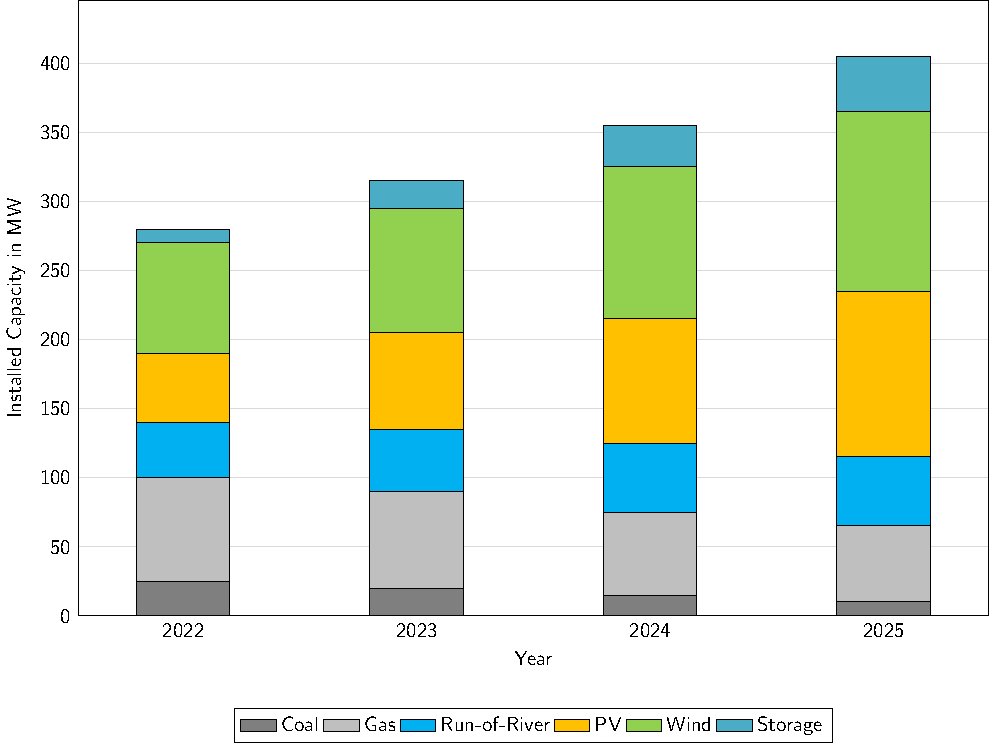
\includegraphics[width=\linewidth]{figures/installed_capacity_2022-2025.pdf}
                    \caption{\centering Installed capacity per power plant type in Wakanda from 2022-2025.}
                    \label{fig:installed_capacity}
            \end{figure}
    
            \onslide<2>\begin{figure}[htbp]
                % Figure generated seperately for faster compilation time. 
                 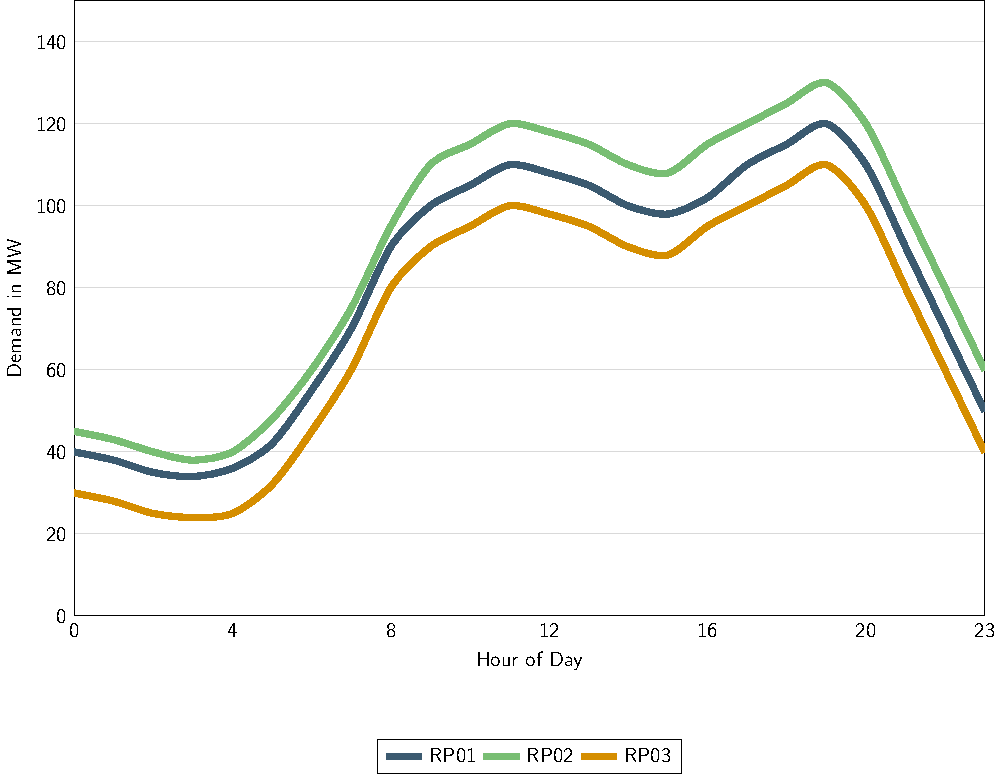
\includegraphics[width=\linewidth]{figures/demand_rp.pdf}  % path to your PDF file
                \caption{\centering Demand per representative periode in Wakanda.}
                \label{fig:demand}
            \end{figure}
     
            \onslide<3>\vspace{-1cm}\begin{figure}[htbp]
                % Figure generated seperately for faster compilation time. 
                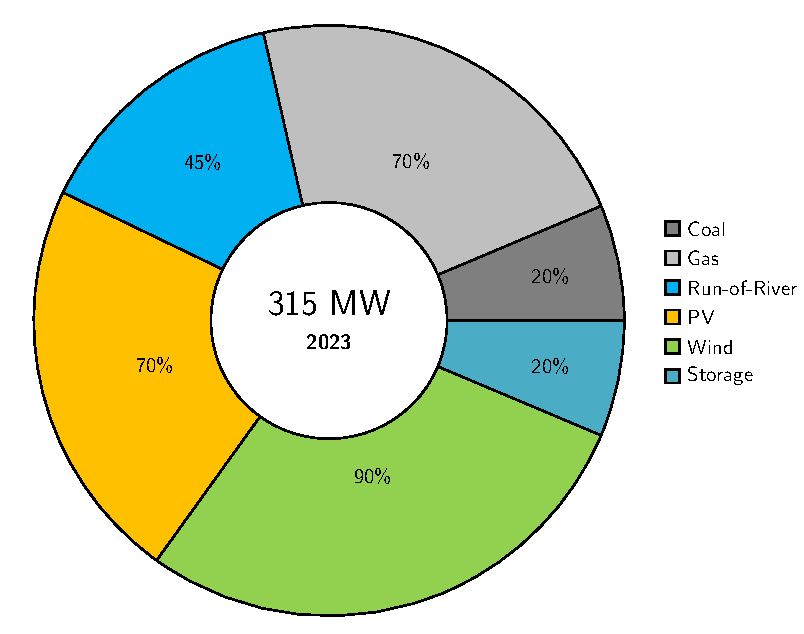
\includegraphics[width=\linewidth]
                {figures/installed_capacity_2023_percent.pdf}  % path to your PDF file
                \caption{\centering Shares of installed capacity per power plant type in Wakanda 2023.}
                \label{fig:installed_capacity_2023}
            \end{figure}
            \end{overprint}
        \end{column}
    \end{columns}

    \addsource{Source: Energy Report, Statistics Wakanda, 2023}
\end{frame}


\begin{frame}{Plots}
    \framesubtitle{Colors for Power Plants}

    \begin{table}[htbp]
        \scalebox{0.94}{
            % ==============================================================================
% Power Plant Colors Table
% ==============================================================================
% This file defines a color-coded table of power plant types using tabularray.
% It can be compiled standalone (for preview/export) or input into a larger LaTeX
% document (e.g., a Beamer presentation).
%
% To compile standalone, set \standalonetrue below.
% To use via \input{}, ensure \standalonefalse is set (default).
% ==============================================================================

\newif\ifstandalone
% \standalonetrue    % Uncomment this line to compile standalone
\standalonefalse     % Default for input into other documents

\ifstandalone
    \documentclass{standalone}
    \usepackage[table]{xcolor}
    \usepackage{tabularray}
    \UseTblrLibrary{booktabs}
    \UseTblrLibrary{siunitx}
    \usepackage{graphicx}
    \usepackage{tikz}
    \usepackage{sfmath}
    \renewcommand{\familydefault}{\sfdefault}

    % Load color definitions (always)
    % TU Graz Colors
\definecolor{tug}{HTML}{F70146}

% IEE Color
\definecolor{iee}{HTML}{008080}
\colorlet{main}{iee}

% PowerPoint Palette
\definecolor{fore}{HTML}{0F0F0F}
\definecolor{back}{HTML}{FFFFFF}
\definecolor{dark}{HTML}{3B5A70}
\definecolor{lite}{HTML}{A6A6A6}
\definecolor{head}{HTML}{245B78}
\definecolor{body}{HTML}{E2E9ED}
\definecolor{urlA}{HTML}{0066D8}
\definecolor{urlB}{HTML}{6C2F91}
\colorlet{colA}{iee}
\colorlet{colB}{tug}
\definecolor{colC}{HTML}{6BA3A3}
\definecolor{colD}{HTML}{2E4172}
\definecolor{colE}{HTML}{78BE73}
\definecolor{colF}{HTML}{D58E00}
\colorlet{grey}{lite}
\colorlet{default}{dark}

% Alternate color names
\colorlet{blue}{dark}
\colorlet{turquoise}{colC}
\colorlet{green}{colE}
\colorlet{yellow}{colF}
\colorlet{red}{colB}

% Light Shades
\definecolor{greyLight}{HTML}{EDEDED}
\definecolor{blueLight}{HTML}{D3DFE8}
\definecolor{ieeLight}{HTML}{E1EDED}
\definecolor{redLight}{HTML}{FFCBDA}
\definecolor{turquoiseLight}{HTML}{E1EDED}
\definecolor{greenLight}{HTML}{E4F2E3}
\definecolor{yellowLight}{HTML}{FFEBC4}

% Dark Shades
\definecolor{greyDark}{HTML}{0F0F0F}
\definecolor{blueDark}{HTML}{1D2D38}
\definecolor{ieeDark}{HTML}{004040}
\definecolor{redDark}{HTML}{7C0023}
\definecolor{turquoiseDark}{HTML}{345353}
\definecolor{greenDark}{HTML}{346830}
\definecolor{yellowDark}{HTML}{6A4700}

% Power Plant Colors
\definecolor{oilColor}{RGB}{16, 47, 64}
\definecolor{coalColor}{RGB}{127, 127, 127}
\definecolor{gasColor}{RGB}{191, 191, 191}
\definecolor{otherNonResColor}{RGB}{221, 110, 56}
\definecolor{nuclearColor}{RGB}{236, 96, 95}
\definecolor{biomassColor}{RGB}{198, 70, 59}
\definecolor{rorColor}{RGB}{0, 176, 240}
\definecolor{pvColor}{RGB}{255, 192, 0}
\definecolor{windColor}{RGB}{146, 208, 80}
\definecolor{windOffColor}{RGB}{30, 143, 79}
\definecolor{otherResColor}{RGB}{185, 207, 222}
\definecolor{storageHydroColor}{RGB}{75, 172, 198}
\definecolor{pumpedStorageColor}{RGB}{59, 90, 112}
\definecolor{bessColor}{RGB}{112, 48, 160}
\definecolor{otherStorageColor}{RGB}{76, 133, 123}

    \begin{document}
\fi

\footnotesize
\centering
\begin{tblr}{
    colspec={lllrrrrc},
    hline{1-2}={solid,1.5pt},
    hline{3-Y}={grey},
    hline{Z}={solid,1.5pt},
    row{odd}={grey!20},
    row{1}={white,font=\bfseries},
    cell{2}{8}={bg=oilColor},
    cell{3}{8}={bg=coalColor},
    cell{4}{8}={bg=gasColor},
    cell{5}{8}={bg=otherNonResColor},
    cell{6}{8}={bg=nuclearColor},
    cell{7}{8}={bg=biomassColor},
    cell{8}{8}={bg=rorColor},
    cell{9}{8}={bg=pvColor},
    cell{10}{8}={bg=windColor},
    cell{11}{8}={bg=windOffColor},
    cell{12}{8}={bg=otherResColor},
    cell{13}{8}={bg=storageHydroColor},
    cell{14}{8}={bg=pumpedStorageColor},
    cell{15}{8}={bg=bessColor},
    cell{16}{8}={bg=otherStorageColor},
}
    \textbf{Power Plant Type} & \textbf{German Name} & \textbf{LaTeX~Name} & \textbf{R} & \textbf{G} & \textbf{B} & \textbf{Hex} & \textbf{Color} \\
    Oil & Öl & \texttt{\textbackslash oilColor} & 16 & 47 & 64 & 102F40 & \\
    Coal & Kohle & \texttt{\textbackslash coalColor} & 127 & 127 & 127 & 7F7F7F &  \\
    Gas & Gas & \texttt{\textbackslash gasColor} & 191 & 191 & 191 & BFBFBF &  \\
    Other non-RES & Sonstige nicht-EE & \texttt{\textbackslash otherNonResColor} & 221 & 110 & 56 & DD6E38 &  \\
    Nuclear & Nuklear & \texttt{\textbackslash nuclearColor} & 236 & 96 & 95 & EC605F &  \\
    Biomass & Biomasse & \texttt{\textbackslash biomassColor} & 198 & 70 & 59 & C6463B &  \\
    Run-of-River & Laufwasserkraft & \texttt{\textbackslash rorColor} & 0 & 176 & 240 & 00B0F0 &  \\
    Solar/PV & Solar/PV & \texttt{\textbackslash pvColor} & 255 & 192 & 0 & FFC000 &  \\
    Wind-onshore & Wind-onshore & \texttt{\textbackslash windColor} & 146 & 208 & 80 & 92D050 &  \\
    Wind-offshore & Wind-offshore & \texttt{\textbackslash windOffColor} & 30 & 143 & 79 & 1E8F4F &  \\
    Other RES & Sonstige EE & \texttt{\textbackslash otherResColor} & 185 & 207 & 222 & B9CFDE &  \\
    Storage Hydro & Wasserspeicher & \texttt{\textbackslash storageHydroColor} & 75 & 172 & 198 & 4BACC6 &  \\
    Pumped Storage & Pumpspeicher & \texttt{\textbackslash pumpedStorageColor} & 59 & 90 & 112 & 3B5A70 &  \\
    BESS & Batteriespeicher & \texttt{\textbackslash bessColor} & 112 & 48 & 160 & 7030A0 &  \\
    Other Storages & Sonstige Speicher & \texttt{\textbackslash otherStorageColor} & 76 & 133 & 123 & 4C857B &  \\
\end{tblr}

\ifstandalone
    \end{document}
\fi

        }
    \end{table}

\end{frame}


%% -------------------------------------------------------------------
%% Structure your Data with Clear Tables
\section{\textbf{Structure} your \textbf{Data} with Clear \textbf{Tables}}

\begin{frame}
    \agenda     
    % Customized agenda:     
    % \agenda[sections=all or currentsection][title][subtitle][picture][picture source]
\end{frame}

\begin{frame}{Tables}
    \framesubtitle{Clear and Well-Designed Tables}

    \vspace{-.7cm}
    \begin{columns}
        \begin{column}{0.49\textwidth}
            \begin{coloredblock}[turquoise][\faIcon{table}~~~Table Design][\footnotesize\centering]
                \vspace{0.2cm}
                \begin{tugitemize}
                    \item \footnotesize \textbf{Bold headers} for clarity and emphasis
                    \item \textbf{Black vertical lines} for \textbf{header} and \textbf{bottom} only (1.5~pt) 
                    \item \textbf{Grey vertical lines} (1~pt) for the \textbf{rest}
                    \item \footnotesize \textbf{Avoid horizontal lines} (unless necessary)
                    \item \footnotesize \textbf{Use gray!20} as \textbf{background} for \textbf{odd rows}
                \end{tugitemize}
            \end{coloredblock}
            \vspace{0.2cm}
            \begin{coloredblock}[yellow][\faIcon{glasses}~~~Data Readability][\footnotesize\centering]
                \vspace{0.2cm}
                \begin{tugitemize}
                    \item \footnotesize \textbf{Align numbers by decimal separator} for better readability
                    \item \footnotesize \textbf{Show only meaningful decimals} – no clutter!
                    \item \footnotesize \textbf{Use consistent units} and place them in the header when possible
                    \item \footnotesize \textbf{Highlight} the numbers you want to emphasize
                \end{tugitemize}
            \end{coloredblock}
        \end{column}
        \begin{column}{0.49\textwidth}
            \vspace{2cm}            
            \begin{table}[htbp]
                % ==============================================================================
% Power Plant Colors Table
% ==============================================================================
% This file defines a color-coded table of power plant types using tabularray.
% It can be compiled standalone (for preview/export) or input into a larger LaTeX
% document (e.g., a Beamer presentation).
%
% To compile standalone, set \standalonetrue below.
% To use via \input{}, ensure \standalonefalse is set (default).
% ==============================================================================

\newif\ifstandalone
% \standalonetrue    % Uncomment this line to compile standalone
\standalonefalse     % Default for input into other documents

\ifstandalone
    \documentclass{standalone}
    \usepackage[table]{xcolor}
    \usepackage{tabularray}
    \UseTblrLibrary{booktabs}
    \UseTblrLibrary{siunitx}
    \usepackage{graphicx}
    \usepackage{tikz}
    \usepackage{sfmath}
    \renewcommand{\familydefault}{\sfdefault}

    % Load color definitions (always)
    % TU Graz Colors
\definecolor{tug}{HTML}{F70146}

% IEE Color
\definecolor{iee}{HTML}{008080}
\colorlet{main}{iee}

% PowerPoint Palette
\definecolor{fore}{HTML}{0F0F0F}
\definecolor{back}{HTML}{FFFFFF}
\definecolor{dark}{HTML}{3B5A70}
\definecolor{lite}{HTML}{A6A6A6}
\definecolor{head}{HTML}{245B78}
\definecolor{body}{HTML}{E2E9ED}
\definecolor{urlA}{HTML}{0066D8}
\definecolor{urlB}{HTML}{6C2F91}
\colorlet{colA}{iee}
\colorlet{colB}{tug}
\definecolor{colC}{HTML}{6BA3A3}
\definecolor{colD}{HTML}{2E4172}
\definecolor{colE}{HTML}{78BE73}
\definecolor{colF}{HTML}{D58E00}
\colorlet{grey}{lite}
\colorlet{default}{dark}

% Alternate color names
\colorlet{blue}{dark}
\colorlet{turquoise}{colC}
\colorlet{green}{colE}
\colorlet{yellow}{colF}
\colorlet{red}{colB}

% Light Shades
\definecolor{greyLight}{HTML}{EDEDED}
\definecolor{blueLight}{HTML}{D3DFE8}
\definecolor{ieeLight}{HTML}{E1EDED}
\definecolor{redLight}{HTML}{FFCBDA}
\definecolor{turquoiseLight}{HTML}{E1EDED}
\definecolor{greenLight}{HTML}{E4F2E3}
\definecolor{yellowLight}{HTML}{FFEBC4}

% Dark Shades
\definecolor{greyDark}{HTML}{0F0F0F}
\definecolor{blueDark}{HTML}{1D2D38}
\definecolor{ieeDark}{HTML}{004040}
\definecolor{redDark}{HTML}{7C0023}
\definecolor{turquoiseDark}{HTML}{345353}
\definecolor{greenDark}{HTML}{346830}
\definecolor{yellowDark}{HTML}{6A4700}

% Power Plant Colors
\definecolor{oilColor}{RGB}{16, 47, 64}
\definecolor{coalColor}{RGB}{127, 127, 127}
\definecolor{gasColor}{RGB}{191, 191, 191}
\definecolor{otherNonResColor}{RGB}{221, 110, 56}
\definecolor{nuclearColor}{RGB}{236, 96, 95}
\definecolor{biomassColor}{RGB}{198, 70, 59}
\definecolor{rorColor}{RGB}{0, 176, 240}
\definecolor{pvColor}{RGB}{255, 192, 0}
\definecolor{windColor}{RGB}{146, 208, 80}
\definecolor{windOffColor}{RGB}{30, 143, 79}
\definecolor{otherResColor}{RGB}{185, 207, 222}
\definecolor{storageHydroColor}{RGB}{75, 172, 198}
\definecolor{pumpedStorageColor}{RGB}{59, 90, 112}
\definecolor{bessColor}{RGB}{112, 48, 160}
\definecolor{otherStorageColor}{RGB}{76, 133, 123}

    \begin{document}
\fi
\centering
\small
\begin{tblr}{
      colspec = {
            l 
            S[table-format=4.1] % S for decimal-aligned numeric columns
            S[table-format=3.1] % S for decimal-aligned numeric columns
            S[table-format=3.1] % S for decimal-aligned numeric columns
            S[table-format=3.1] % S for decimal-aligned numeric columns
      },
      hline{1-2}={solid,1.5pt}, % Header with black lines on top and bottom
      hline{3-Y}={grey}, % Grey lines between rows
      hline{Z}={solid,1.5pt}, % Black line at the end
      row{odd}={grey!20}, % Background color odd rows
      % row{even}={white}, % Background color even rows
      row{1}={white,font=\bfseries}, % Bold font for header
      cell{4}{2}={yellowLight, cmd=\textbf}, % Highlight cell (has to be after row{odd}={grey!20})
      cell{4}{3}={yellowLight, cmd=\textbf}, % Highlight cell (has to be after row{odd}={grey!20})
    }
    \textbf{Power Plant Type} & \textbf{2022} & \textbf{2023} & \textbf{2024} & \textbf{2025} \\
    Coal           & 25.3 & 20.6 & 15.9 & 10.5 \\
    Gas            & 75.3 & 70.5 & 60.2 & 55.6 \\
    Run-of-River   & 40.3 & 45.0 & 50.0 & 50.0 \\
    PV             & 50.5 & 70.5 & 90.7 & 120.0 \\
    Wind           & 80.0 & 90.2 & 110.3 & 130.4 \\
    Storage Hydro  & 10.7 & 20.0 & 30.7 & 40.2 \\
\end{tblr}

\ifstandalone
    \end{document}
\fi

                \caption{\centering Installed capacity per power plant type in Wakanda from 2022--2025 in MW.}
            \end{table}
        \end{column}
    \end{columns}

    \addsource{Source: Energy Report, Statistics Wakanda, 2023}
    
\end{frame}


%% -------------------------------------------------------------------
%% Additional Tips to Improve your Design
\section{Additional \textbf{Tips} to Improve your Design}

\begin{frame}
    \agenda     
    % Customized agenda:     
    % \agenda[sections=all or currentsection][title][subtitle][picture][picture source]
\end{frame}

\begin{frame}{Additional Tips}
    \framesubtitle{Improve your Design}

    \begin{coloredblock}[iee][\faIcon{dog}~~~Icon][\centering]
        \begin{itemize}
            \item Incorporate \textbf{icons} to enhance \textbf{visual clarity and aid }quick \textbf{comprehension}
            \item The \textbf{recommended option} in \LaTeX~is to use icons from the \textbf{fontawesome package}. You can find all \textbf{available icons} in the \href{https://mirror.easyname.at/ctan/fonts/fontawesome5/doc/fontawesome5.pdf}{\textbf{docs}}. Add an attribution on the \hyperlink{frame:closing_slide}{closing slide}.

            \item When using \textbf{third-party icons}:
            \vspace{-0.5\topsep}
            \begin{itemize}
                \item Ensure the icons follow a \textbf{consistent design} style
                \item Verify that you have the appropriate \textbf{usage rights} for the icons
            \end{itemize}
        \end{itemize}
    \end{coloredblock}

        \begin{coloredblock}[yellow][\faIcon{image}~~~Pictures][\centering]
            \begin{itemize}
                \item Always \textbf{credit} the \textbf{source} of your pictures. Use the function \texttt{\textbackslash addsource\{\}}.
                \item Ensure all images are \textbf{crisp} and \textbf{sharp} for \textbf{optimal quality}
            \end{itemize}
        \end{coloredblock}
\end{frame}

\begin{frame}{Faded Image}
    \framesubtitle{Add a Nice Visual Touch}

    \vspace{.6cm}
    \insertfadedpicture{15.98cm}{figures/iee_besprechung.png}{Source: Institute of Electricity Economics and Energy Innovation/TU Graz}

        \begin{coloredblock}[blue][\faIcon{image}~~~Faded Image][\centering ][][][.75\textwidth]
            \begin{itemize}
               \item To \textbf{add} a \textbf{faded image} as a background to your slide, use the \textbf{following command}:
                \item[] \begin{center}\footnotesize\texttt{\textbackslash insertfadedpicture\{inset from right\}\{image path\}\{Optional: caption text\}}\end{center}
                \begin{itemize}
                    \item \textbf{Inset from right}: Defines how far the image should be shifted in from the right edge. (Ensure the image is large enough.)
                    \item \textbf{Image path}: Specifies the file path to the image.
                    \item \textbf{Caption text}: Provides the text (e.g., image source) to be displayed in the bottom-right corner.
                \end{itemize}
                \item This \textbf{must be included at the beginning} of your \textbf{frame}.
            \end{itemize}     
        \end{coloredblock}

\end{frame}


\begin{frame}{Lists}
    \framesubtitle{Different Styles of Lists}

    \begin{coloredblock}[yellow]
        \centering
        There are \textbf{different styles} of \textbf{lists} that you can choose from.
    \end{coloredblock}

    \vspace{-0.5cm}

    % Bottom blocks (side-by-side)
    \begin{columns}
        \begin{column}{0.49\textwidth}
            \begin{coloredblock}[blue][\texttt{\textbf{\textbackslash begin\{itemize\}}}:][\footnotesize\centering][][4.5cm]
                \begin{itemize}
                    \item Item level 1
                    \begin{itemize}
                        \item Item level 2
                        \begin{itemize}
                            \item Item level 3
                        \end{itemize}
                    \end{itemize}
                \end{itemize}
            \end{coloredblock}
    
            \begin{coloredblock}[iee][\texttt{\textbf{\textbackslash begin\{enumerate\}}}:][\footnotesize\centering][][4.5cm]
                \begin{enumerate}
                \item Item level 1
                    \begin{enumerate}
                        \item Item level 2
                        \begin{enumerate}
                            \item Item level 3
                        \end{enumerate}
                    \end{enumerate}
                \end{enumerate}
            \end{coloredblock}
        \end{column}
        
        \begin{column}{0.49\textwidth}
            \begin{coloredblock}[green][\texttt{\textbackslash begin\{tugitemize\}} (tighter spacing):][\footnotesize\centering][][4.5cm]
                \vspace{0.5cm}
                \begin{tugitemize}
                    \item Item level 1
                    \begin{tugitemize}
                        \item Item level 2
                        \begin{tugitemize}
                            \item Item level 3
                        \end{tugitemize}
                    \end{tugitemize}
                \end{tugitemize}
            \end{coloredblock}
    
            \begin{coloredblock}[grey][\texttt{\textbackslash begin\{tugenumerate\}} (tighter spacing):][\footnotesize\centering][][4.5cm]
                \vspace{0.5cm}
                \begin{tugenumerate}
                    \item Item level 1
                    \begin{tugenumerate}
                        \item Item level 2
                        \begin{tugenumerate}
                            \item Item level 3
                        \end{tugenumerate}
                    \end{tugenumerate}
                \end{tugenumerate}
            \end{coloredblock}
        \end{column}
    \end{columns}
\end{frame}


\begin{frame}{Lists}
    \framesubtitle{Different Styles of Lists}

    \begin{coloredblock}[yellow]
        \centering
        There are \textbf{different styles} of \textbf{lists} that you can choose from.
    \end{coloredblock}

    \vspace{-0.5cm}

    % Bottom blocks (side-by-side)
    \begin{columns}
        \begin{column}{0.49\textwidth}
            \begin{coloredblock}[turquoise][\texttt{\textbf{\textbackslash begin\{romanenumerate\}}}:][\footnotesize\centering][][4.5cm]
                \begin{romanenumerate}
                    \item Item level 1
                    \begin{romanenumerate}
                        \item Item level 2
                        \begin{romanenumerate}
                            \item Item level 3
                        \end{romanenumerate}
                    \end{romanenumerate}
                \end{romanenumerate}
            \end{coloredblock}
    
            \begin{coloredblock}[yellow][\texttt{\textbf{\textbackslash begin\{boxenumerate\}}}:][\footnotesize\centering][][4.5cm]
                \begin{boxenumerate}
                \item Item level 1
                    \begin{boxenumerate}
                        \item Item level 2
                        \begin{boxenumerate}
                            \item Item level 3
                        \end{boxenumerate}
                    \end{boxenumerate}
                \end{boxenumerate}
            \end{coloredblock}
        
        \end{column}
        \begin{column}{0.49\textwidth}
            \begin{coloredblock}[blue][\texttt{\textbackslash begin\{tugromanenumerate\}} (tighter spacing):][\footnotesize\centering][][4.5cm]
                \vspace{0.5cm}
                \begin{tugromanenumerate}
                    \item Item level 1
                    \begin{tugromanenumerate}
                        \item Item level 2
                        \begin{tugromanenumerate}
                            \item Item level 3
                        \end{tugromanenumerate}
                    \end{tugromanenumerate}
                \end{tugromanenumerate}
            \end{coloredblock}
    
            \begin{coloredblock}[red][\texttt{\textbackslash begin\{boxromanenumerate\}}:][\footnotesize\centering][][4.5cm]
                    \begin{boxromanenumerate}
                        \item Item level 1
                        \begin{boxromanenumerate}
                            \item Item level 2
                            \begin{boxromanenumerate}
                                \item Item level 3
                            \end{boxromanenumerate}
                        \end{boxromanenumerate}
                    \end{boxromanenumerate}
            \end{coloredblock}
        \end{column}
    \end{columns}
\end{frame}


%% -------------------------------------------------------------------
%% Acknowledge Work with Proper Citations
\section{\textbf{Acknowledge} Work with Proper \textbf{Citations}}

\begin{frame}
    \agenda     
    % Customized agenda:     
    % \agenda[sections=all or currentsection][title][subtitle][picture][picture source]
\end{frame}


\begin{frame}{References}
    \framesubtitle{Cite the Sources you use}

    \begin{coloredblock}[grey]
        \centering
        ”\textit{In the middle of every difficulty lies opportunity.}“
          
        \vspace{0.7cm}
        \scriptsize A. Einstein \cite{einstein2018}
    \end{coloredblock}
    
    \begin{coloredblock}[blue][\centering\texttt{\textbackslash textcite\{\}}]
        If you want to include the authors, use \texttt{\textbackslash textcite\{\}}.
    
        \vspace{0.5cm}
        In their study, \textbf{\textcite{gaugl2023}} demonstrate that rising CO\textsubscript{2} prices result in higher electricity prices in Austria.
    \end{coloredblock}
    
    \begin{coloredblock}[yellow][\centering\texttt{\textbackslash cite\{\}}]
        A simple reference is accomplished with \texttt{\textbackslash cite\{\}}.
    
        \vspace{0.5cm}
        The LEGO model is an energy system optimization model developed at the Institute of Electricity Economics and Energy Innovation. \textbf{\cite{wogrin2022}}
    \end{coloredblock}

\end{frame}


%% -------------------------------------------------------------------
%% Explore Design Inspirations to Spark  your Creativity
\section{Explore \textbf{Design Inspirations} to Spark  your Creativity}

\begin{frame}
    \agenda     
    % Customized agenda:     
    % \agenda[sections=all or currentsection][title][subtitle][picture][picture source]
\end{frame}

% Slide with big Title and Subtitle \sectionheader[Subtitle]{Title}
\sectionheader[Spark your Creativity]{Design Inspirations}


\begin{frame}{Methodology}
    \framesubtitle{NTC Model}

    \begin{minipage}[t]{0.2\textwidth}
        \begin{coloredblockdark}[blue][][][][2.35cm][][0ex][0ex]
                \begin{minipage}[c][2.35cm][c]{0.4\textwidth}
                    \centering
                    \Large{\faIcon{coins}}
                \end{minipage}%
                \hfill
                \begin{minipage}[c][2.35cm][c]{0.55\textwidth}
                    \centering
                    \tiny\textbf{Objective Function:}\\
                    Minimize total system costs
                \end{minipage}%
                \hspace{0.05\textwidth}
        \end{coloredblockdark}
        \vspace{-0.55cm}
        \begin{coloredblockdark}[blue][][][][2.35cm][][0ex][0ex]
                \begin{minipage}[c][2.35cm][c]{0.4\textwidth}
                    \centering
                    \Large{\faIcon{balance-scale}}
                \end{minipage}%
                \hfill
                \begin{minipage}[c][2.35cm][c]{0.55\textwidth}
                    \centering
                    \tiny\textbf{Constraint 1:}\\ 
                    Balance equation
                \end{minipage}%
                \hspace{0.05\textwidth}
        \end{coloredblockdark}
        \vspace{-0.55cm}
        \begin{coloredblockdark}[blue][][][][2.35cm][][0ex][0ex]
                \begin{minipage}[c][2.35cm][c]{0.4\textwidth}
                    \centering
                    \Large{\faIcon{hand-paper}}
                \end{minipage}%
                \hfill
                \begin{minipage}[c][2.35cm][c]{0.55\textwidth}
                    \centering
                    \tiny\textbf{Constraint 2:}\\ 
                    NTC Limits
                \end{minipage}%
                \hspace{0.05\textwidth}
        \end{coloredblockdark}
        \vspace{-0.55cm}
        \begin{coloredblockdark}[blue][][][][2.35cm][][0ex][0ex]
                \begin{minipage}[c][2.35cm][c]{0.4\textwidth}
                    \centering
                    \Large{\faIcon{arrows-alt-v}}
                \end{minipage}%
                \hfill
                \begin{minipage}[c][2.35cm][c]{0.55\textwidth}
                    \centering
                    \tiny\textbf{Constraint 3:}\\ 
                    Flow Direction
                \end{minipage}%
                \hspace{0.05\textwidth}
        \end{coloredblockdark}
        \vspace{-0.55cm}
        \begin{coloredblockdark}[blue][][][][2.35cm][][0ex][0ex]
                \begin{minipage}[c][2.35cm][c]{0.4\textwidth}
                    \centering
                    \Large{\faIcon{arrows-alt-h}}
                \end{minipage}%
                \hfill
                \begin{minipage}[c][2.35cm][c]{0.55\textwidth}
                    \centering
                    \tiny\textbf{Constraint 4:}\\ 
                    Export/Import
                \end{minipage}%
                \hspace{0.05\textwidth}
        \end{coloredblockdark}
        \vspace{-0.55cm}
        \begin{coloredblockdark}[blue][][][][2.35cm][][0ex][0ex]
                \begin{minipage}[c][2.35cm][c]{0.4\textwidth}
                    \centering
                    \Large{\faIcon{power-off}}
                \end{minipage}%
                \hfill
                \begin{minipage}[c][2.35cm][c]{0.55\textwidth}
                    \centering
                    \tiny\textbf{Constraint 5:}\\ 
                    Generator Limits
                \end{minipage}%
                \hspace{0.05\textwidth}
        \end{coloredblockdark}
    \end{minipage}
    \hfill
    \begin{minipage}[t]{0.78\textwidth}
        \begin{coloredblock}[blue][][][c][2.35cm][][0ex][0ex]
            \begin{center}
                \footnotesize$\min \sum_{g,h} c_{g}^{op} \cdot p_g^{h} + \sum_{g} x_g \cdot (c_{g}^{Inv,MW} + c_{g}^{Inv,MWh} \cdot E2P_g)$
            \end{center}
        \end{coloredblock}
        \vspace{-0.55cm}
        \begin{coloredblock}[blue][][][c][2.35cm][][0ex][0ex]
            \begin{minipage}[t]{.89\textwidth}
                \begin{center}
                    \footnotesize$\sum_{g} p_{gz(g,z),h} - \sum_{g} p_{cs(g,z),h} - \sum_{z \neq y} exp_{z,y,h} + \sum_{z \neq y} imp{z,y,h} = dem_{z,h}$
                \end{center}
            \end{minipage}
            \hfill
            \begin{minipage}[t]{.1\textwidth}
                \footnotesize $\forall z,y,h$
            \end{minipage}
        \end{coloredblock}
        \vspace{-0.55cm}
        \begin{coloredblock}[blue][][][c][2.35cm][][0ex][0ex]
            \begin{minipage}[t]{.89\textwidth}
                \begin{center}
                    \footnotesize$exp_{z,y,h} \leq NTC_{z,y} \cdot bn_{z,y,h}$
                \end{center}
            \end{minipage}
            \hfill
            \begin{minipage}[t]{.1\textwidth}
                \footnotesize $\forall z,y,h$
            \end{minipage}
        \end{coloredblock}
        \vspace{-0.55cm}
        \begin{coloredblock}[blue][][][c][2.35cm][][0ex][0ex]
            \begin{minipage}[t]{.89\textwidth}
                \begin{center}
                    \footnotesize$imp_{z,y,h} \leq NTC_{y,z} \cdot (1-bn_{z,y,h})$
                \end{center}
            \end{minipage}
            \hfill
            \begin{minipage}[t]{.1\textwidth}
                \footnotesize $\forall z,y,h$
            \end{minipage}
        \end{coloredblock}
        \vspace{-0.55cm}
        \begin{coloredblock}[blue][][][c][2.35cm][][0ex][0ex]
            \begin{minipage}[t]{.89\textwidth}
                \begin{center}
                    \footnotesize$exp_{z,y,h} = imp_{y,z,h}$
                \end{center}
            \end{minipage}
            \hfill
            \begin{minipage}[t]{.1\textwidth}
                \footnotesize $\forall z,y,h$
            \end{minipage}
        \end{coloredblock}
        \vspace{-0.55cm}
        \begin{coloredblock}[blue][][][c][2.35cm][][0ex][0ex]
            \begin{minipage}[t]{.89\textwidth}
                \begin{center}
                    \footnotesize$\underline{p_g} \leq p_{g,h} \leq \overline{p_g}$
                \end{center}
            \end{minipage}
            \hfill
            \begin{minipage}[t]{.1\textwidth}
                \footnotesize $\forall g,h$
            \end{minipage}
        \end{coloredblock}
    \end{minipage}
    
\end{frame}


\begin{frame}{Decarbonization}
    \framesubtitle{Energy Sectors}

    \vspace{-.9cm}
    \begin{columns}
        \begin{column}{0.587\textwidth}
            \begin{coloredblock}[turquoise][][][c][13.7cm]
                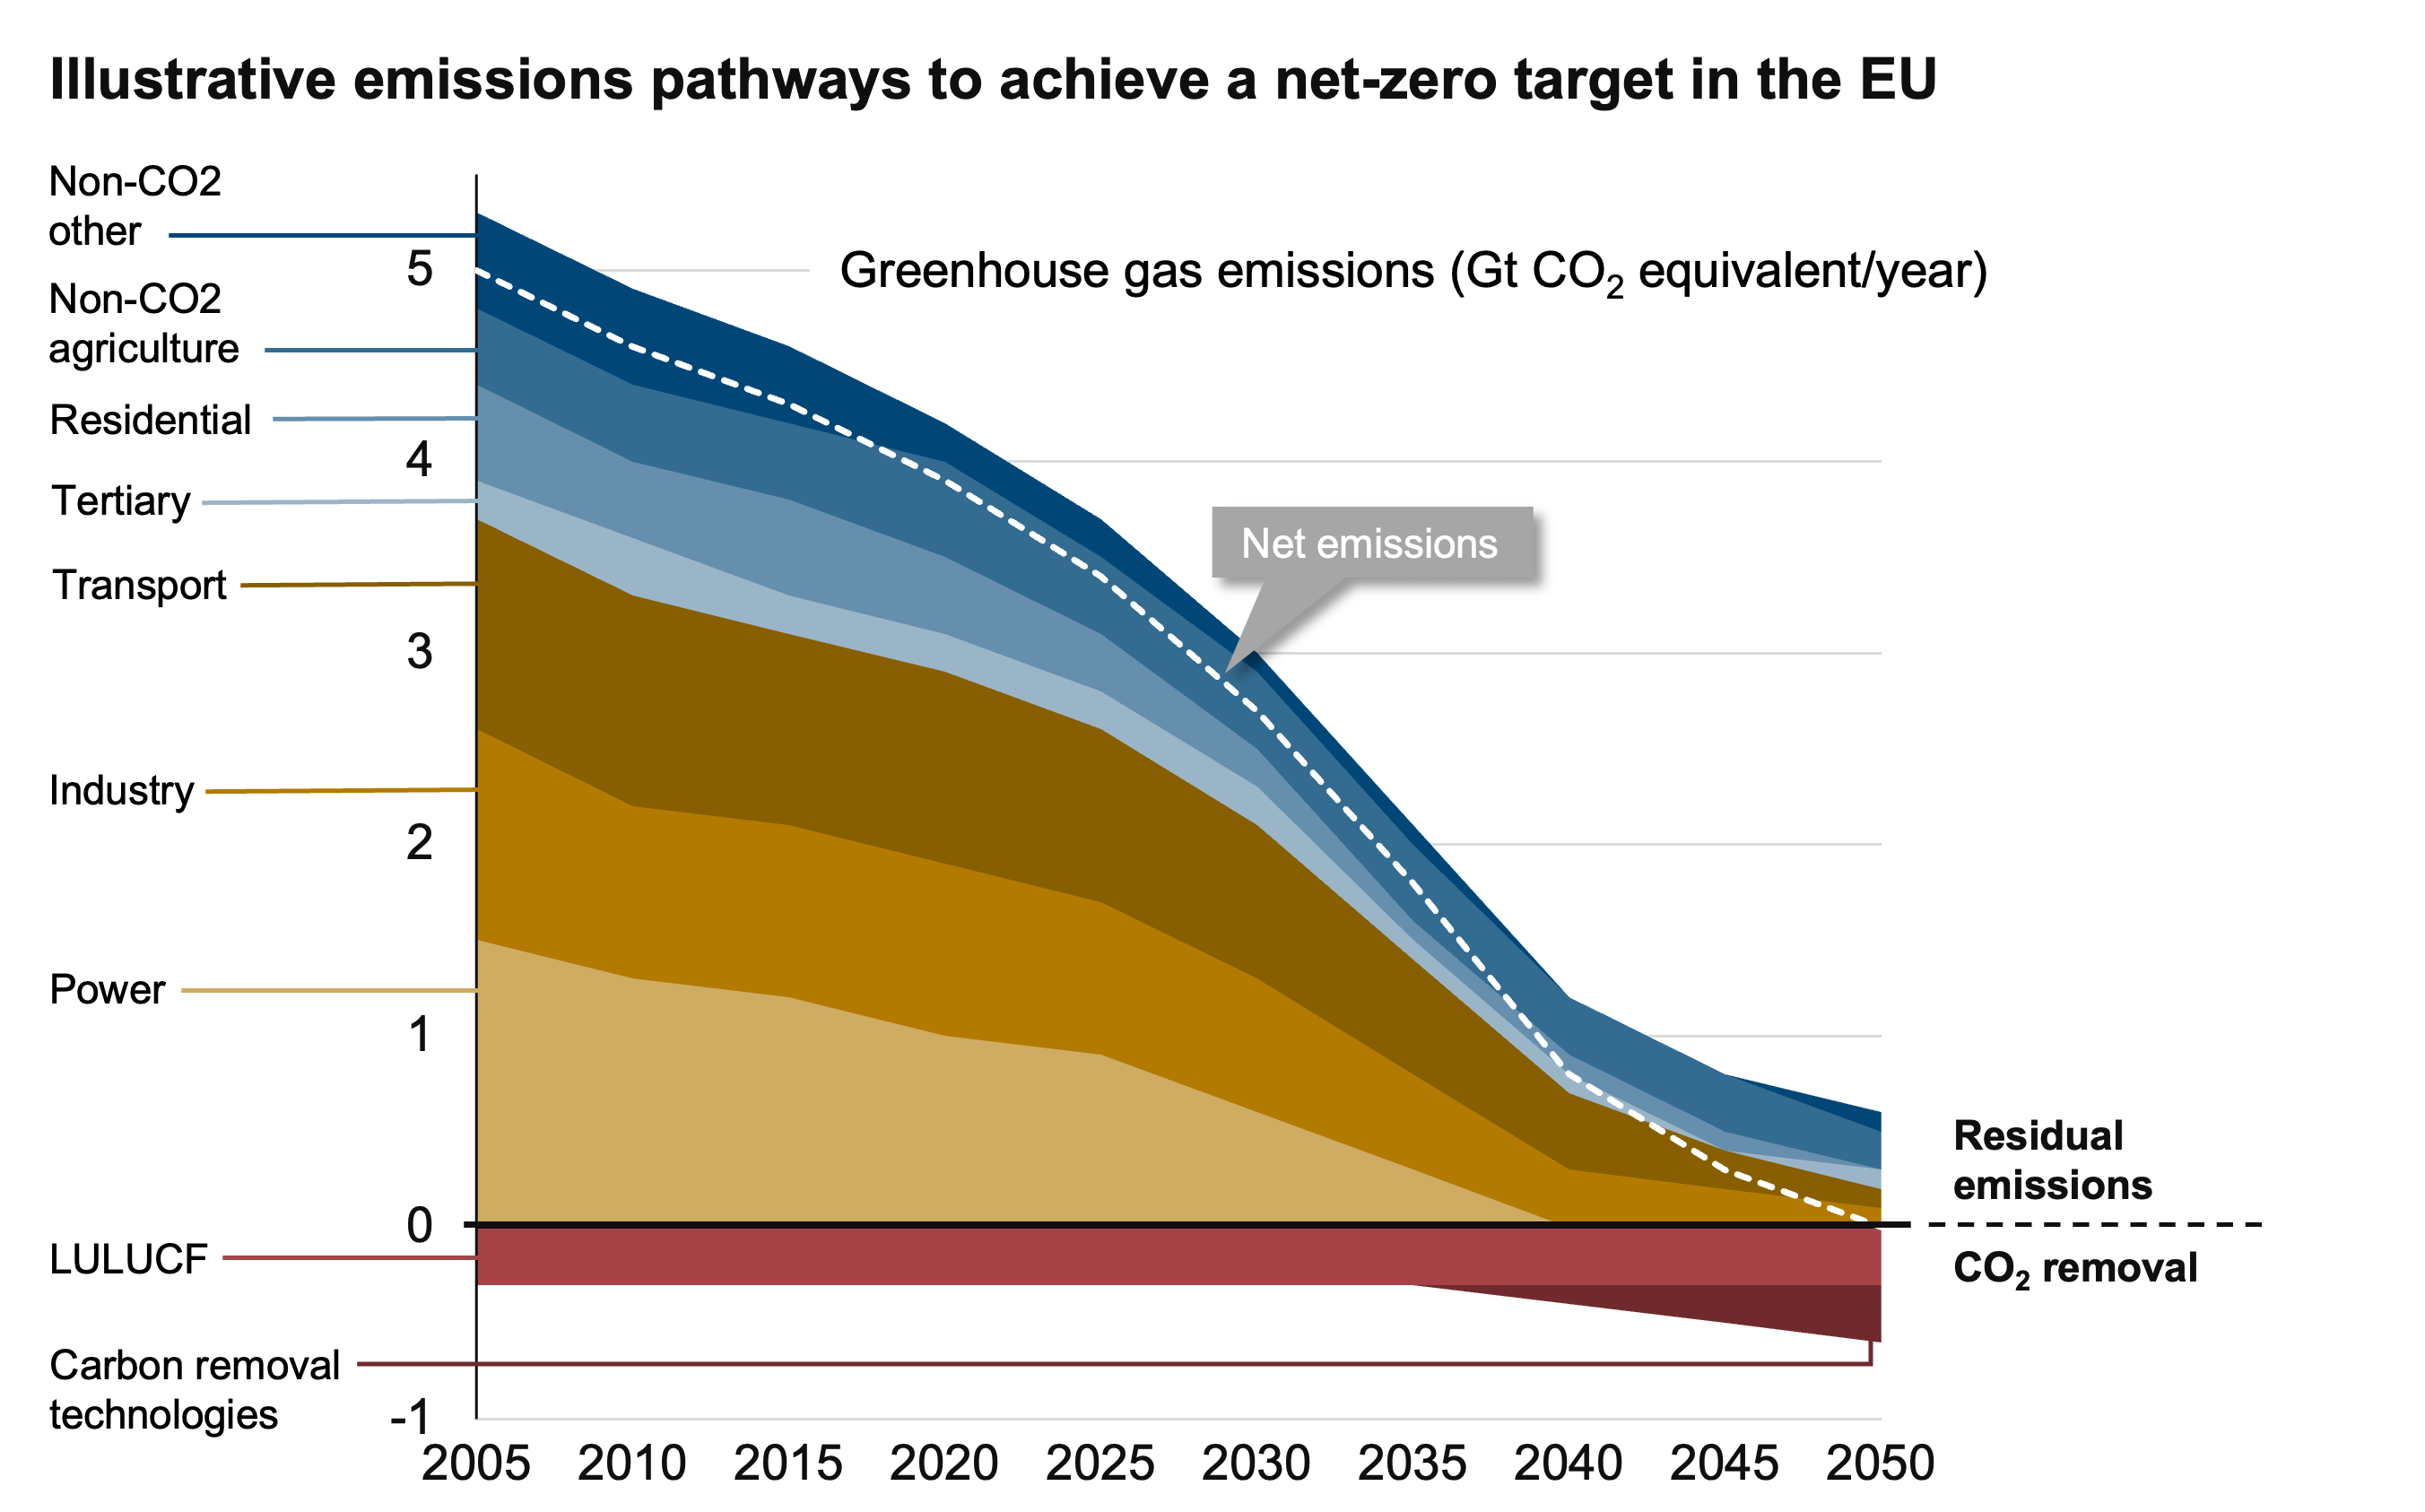
\includegraphics[width=\linewidth]{figures/Path_net-zero.png}
            \end{coloredblock}
        \end{column}
        \begin{column}{0.39\textwidth}
            \begin{coloredblockicon}[grey][][][\large\faIcon{thermometer-half}][l][c][3.7cm]
                \small The European Commission wants to achieve \textbf{climate neutrality until 2050}
            \end{coloredblockicon}
            \begin{coloredblockicon}[grey][][][\large\faIcon{industry}][l][c][5.7cm]
                \small Affected sectors:
                \begin{tugitemize}
                    \item \footnotesize Electric power sector
                    \item \footnotesize Transport and mobility
                    \item \footnotesize Heat
                    \item \footnotesize Gas (hydrogen), etc.
                \end{tugitemize}
            \end{coloredblockicon}
            \begin{coloredblockicon}[grey][][][\large\faIcon{euro-sign}][l][c][3.7cm]
                \small \textbf{Large-scale investments} in (energy) infrastructure required
            \end{coloredblockicon}
        \end{column}
    \end{columns}

    \begin{coloredblock}[yellow][][][c][1.5cm]
        \centering \textbf{Simulation/optimization models} serve as \textbf{decision support tool}.
    \end{coloredblock}

    \addsource{Source: SWP Berlin}

\end{frame}

\begin{frame}{Examined Main Scenarios}
    \framesubtitle{Analysis of Flexibility Requirements}

    \vspace{-.9cm}
    \begin{columns}
        \begin{column}{0.32\textwidth}
            \begin{coloredblock}[green][Scenario\\LOW ENERGY][\footnotesize\centering ]
                \begin{minipage}[t][5cm]{0.9\textwidth} 
                    \scriptsize STORYLINE: Austria continues to face a \textbf{challenging economic situation}, with \textbf{slowed investments} and \textbf{subdued economic growth}:
                \end{minipage}
                \begin{minipage}[t][4.2cm]{0.9\textwidth}
                    \begin{itemize}
                        \item \scriptsize \textbf{Investments} in \textbf{renewable energy} remain \textbf{low}, and \textbf{electricity demand} is \textbf{lower} than projected in the \textbf{ÖNIP} scenario.

                    \end{itemize}
                \end{minipage}
            \end{coloredblock}
        \end{column}
        \begin{column}{0.32\textwidth}
            \begin{coloredblock}[yellow][Scenario\\BASE][\footnotesize\centering ]
                \begin{minipage}[t][5cm]{0.9\textwidth} 
                    \scriptsize STORYLINE: Austria pursues a \textbf{highly ambitious path} to \textbf{decarbonization} and achieves the goal of decarbonization \textbf{by 2040}:
                \end{minipage}
                \begin{minipage}[t][4.2cm]{0.9\textwidth}
                    \begin{itemize}
                        \item \scriptsize Ambitious renewable energy expansion \textbf{aligned with the ÖNIP} (Austrian National Energy and Climate Plan).
                    \end{itemize}
                \end{minipage}
            \end{coloredblock}
        \end{column}
        \begin{column}{0.32\textwidth}
            \begin{coloredblock}[blue][Scenario\\ HIGH ENERGY][\footnotesize\centering ]
                \begin{minipage}[t][5cm]{0.9\textwidth} 
                    \scriptsize STORYLINE: \textbf{Investments} in \textbf{renewable energy exceed expectations}, accompanied by a \textbf{rapid pace} of \textbf{electrification}:
                \end{minipage}
                \begin{minipage}[t][4.2cm]{0.9\textwidth}
                    \begin{itemize}
                        \item \scriptsize This leads to \textbf{increased investments} in \textbf{renewables} and a \textbf{rising electricity demand}.
                    \end{itemize}
                \end{minipage}
            \end{coloredblock}
        \end{column}
    \end{columns}

    \vspace{0.2cm}
    \begin{coloredblock}[grey]
        \centering
        \footnotesize\textbf{Through the in-depth analysis of the BASE scenario and the comparison with the extreme scenarios, the research questions are answered.}
    \end{coloredblock}

\end{frame}


\begin{frame}{Grading}

    \begin{coloredblock}[turquoise]
        \centering\footnotesize\textbf{Attendance mandatory\textsuperscript{1}}
    \end{coloredblock}

    \vspace{-0.5cm}
    \begin{columns}
        \begin{column}{0.32\textwidth}
            \begin{coloredblock}[blue][Participation][\footnotesize\centering][][6.5cm]
                \begin{itemize}
                    \item \footnotesize \textbf{Preparatory tasks}\\
                    Short tasks before class like watching a video, reading a text and answering some questions in TeachCenter
                    \item \footnotesize \textbf{Exercises during class}
                \end{itemize}
            \end{coloredblock}
            \vspace{-.3cm}
            \centering \footnotesize \textbf{50 Point}
        \end{column}
        \begin{column}{0.32\textwidth}
            \begin{coloredblock}[blue][Homework 1][\footnotesize\centering][][6.5cm]
                \begin{itemize}
                    \item \footnotesize \textbf{Exercise}\\
                    Work you have to do at home.
                    \item \footnotesize \textbf{Report}\\
                    Comment your code and write a small report
                \end{itemize}
            \end{coloredblock}
            \vspace{-.3cm}
            \centering \footnotesize \textbf{25 Point}
        \end{column}
        \begin{column}{0.32\textwidth}
            \begin{coloredblock}[blue][Homework 2][\footnotesize\centering][][6.5cm]
                \begin{itemize}
                    \item \footnotesize \textbf{Exercise}\\
                    Work you have to do at home.
                    \item \footnotesize \textbf{Report}\\
                    Comment your code and write a small report
                \end{itemize}
            \end{coloredblock}
            \vspace{-.3cm}
            \centering \footnotesize \textbf{25 Point}
        \end{column}
    \end{columns}
    \vspace{0.7cm}
    \begin{coloredblock}[yellow]
        \centering\footnotesize\textbf{In each part more than 50\% of the points are required for a positive grade}
    \end{coloredblock}

    \vspace{0.2cm}
    \begin{coloredblock}[green]
        \begin{minipage}[c]{0.24\textwidth}
            \centering\footnotesize \textbf{Grading Scale}
        \end{minipage}
        \hfill
        \begin{minipage}[c]{0.24\textwidth}
            \footnotesize
            <50 Points:         5\\
            50 – 62 Points:     4
        \end{minipage}
        \hfill
        \begin{minipage}[c]{0.24\textwidth}
            \footnotesize
            63 – 75 Points:     3\\
            76 – 88 Points:     2
        \end{minipage}
        \hfill
        \begin{minipage}[t]{0.24\textwidth}
            \footnotesize
            89 – 100 Points:    1
        \end{minipage}
        
    \end{coloredblock}

    \addsource{\textsuperscript{1} If more than two lessons are missed without an adequate excuse, you can no longer successfully complete the course.}

\end{frame}


\begin{frame}{Classification}
    \framesubtitle{Definition}
    \small\centering\textbf{Classification} is a \textbf{machine learning technique} used to \textbf{predict group membership} for data instances.

    \vspace{.3cm}
    \begin{coloredblockicon}[yellow][Training Data][\footnotesize][\faIcon{table}]
        \vspace{.3cm}
        \begin{tugitemize}
            \item \scriptsize Given a collection of \textbf{records (training set)}, each record contains a set of \textbf{attributes}, with one attribute being the \textbf{class}.
            \item \scriptsize Each sample is characterized by a \textbf{tuple (X, y)}, where:
            \vspace{-.3cm}
            \begin{tugitemize}
                \item \scriptsize \textbf{X: attribute set (predictor, independent variable, input)}
                \item \scriptsize \textbf{y: class label (response, dependent variable, output)}
            \end{tugitemize}
        \end{tugitemize}
    \end{coloredblockicon}

    \begin{coloredblockicon}[green][Task][\footnotesize][\faIcon{tasks}]
        \vspace{.3cm}
        \begin{tugitemize}
            \item \scriptsize Learn a \textbf{model} that maps each \textbf{attribute set X} to one of the predefined \textbf{class labels y}.
            \item \scriptsize Find a \textbf{model} for the \textbf{class attribute} as a \textbf{function} of the values of other attributes.
        \end{tugitemize}
    \end{coloredblockicon}

    \begin{coloredblockicon}[blue][Goal][\footnotesize][\faIcon{bullseye}]
        \vspace{.3cm}
        \begin{tugitemize}
            \item \scriptsize Assign \textbf{previously unseen records} to a \textbf{class} as \textbf{accurately} as possible.
            \item \scriptsize Use a \textbf{test set} to determine the \textbf{accuracy} of the model.
            \item \scriptsize Typically, the \textbf{dataset} is \textbf{divided} into \textbf{training} and \textbf{test sets}:
            \vspace{-.3cm}
            \begin{tugitemize}
                \item \scriptsize \textbf{Training set}: Used to \textbf{build} the model
                \item \scriptsize \textbf{Test set}: Used to \textbf{validate} the model
            \end{tugitemize}
        \end{tugitemize}
    \end{coloredblockicon}

\end{frame}


\begin{frame}{Classification}
    \framesubtitle{Examples}

    \vspace{-1cm}
    \begin{columns}
        \begin{column}{0.32\textwidth}
        
            \begin{coloredblock}[yellow][\faIcon[regular]{smile-beam}~~~Sentiment Analysis][\footnotesize\centering][][6.2cm]
                \begin{itemize}
                    \item \scriptsize \textbf{Task}: Determine the sentiment of a text (e.g., reviews, social media posts).
                    \item \scriptsize \textbf{Attributes}: Text data (words, phrases).
                    \item \scriptsize \textbf{Class Labels}: "Pos," "Neg," or "Neutr"
                \end{itemize}
            \end{coloredblock}
            \vspace{0.1cm}
            \begin{coloredblock}[red][\faIcon{image}~~~Image Recognition][\footnotesize\centering][][6.2cm]
                    \begin{itemize}
                        \item \scriptsize \textbf{Task}: Identify objects or people in images.
                        \item \scriptsize \textbf{Attributes}: Pixel values, image features, etc.
                        \item \scriptsize \textbf{Class Labels}: "Cat," "Dog," etc.
                    \end{itemize}
            \end{coloredblock}
            
        \end{column}
        \begin{column}{0.32\textwidth}
            \begin{coloredblock}[blue][\faIcon{stethoscope}~~~Disease Diagnosis][\footnotesize\centering][][6.2cm]
                \begin{itemize}
                    \item \scriptsize \textbf{Task}: Diagnose whether a patient has a particular disease.
                    \item \scriptsize \textbf{Attributes}: Medical history, test results, symptoms.
                    \item \scriptsize \textbf{Class Labels}: "Disease" / "No Disease"
                \end{itemize}
            \end{coloredblock}
            \vspace{0.1cm}
            \begin{coloredblock}[turquoise][\faIcon{comments}~~~Language Detection][\footnotesize\centering][][6.2cm]
                \begin{itemize}
                    \item \scriptsize \textbf{Task}: Identify the language of a given text.
                    \item \scriptsize \textbf{Attributes}: Text data (words, characters).
                    \item \scriptsize \textbf{Class Labels}: "English," "Spanish," etc.
                \end{itemize}
            \end{coloredblock}
        
        \end{column}
        \begin{column}{0.32\textwidth}
        
        \begin{coloredblock}[green][\faIcon{running}~~~Activity Recognition][\footnotesize\centering][][6.2cm]
            \begin{itemize}
                \item \scriptsize \textbf{Task}: Determine the activity being performed based on sensor data.
                \item \scriptsize \textbf{Attributes}: Sensor readings (e.g., from a smartphone or wearable device).
                \item \scriptsize \textbf{Class Labels}: “Biking," "Running,"
            \end{itemize}
        \end{coloredblock}
        \vspace{0.1cm}
        \begin{coloredblock}[grey][\faIcon{envelope}~~~E-Mail Spam Detection][\footnotesize\centering][][6.2cm]
            \begin{itemize}
                \item \scriptsize \textbf{Task}: Classify as "spam" or "not spam."
                \item \scriptsize \textbf{Attributes}: Email content, sender, attachements etc.
                \item \scriptsize \textbf{Class Labels}: "Spam" or "Not Spam"
            \end{itemize}
        \end{coloredblock}
        
        \end{column}
    \end{columns}

\end{frame}


\begin{frame}{Pipeline Gas Transmission}
    \framesubtitle{Framework for Piecewise Linearization}

    \vspace{-.9cm}
    \begin{columns}
        \begin{column}{.39\textwidth}
            \begin{coloredblock}[yellow][][][c][3.5cm]
                \begin{center}
                    \textbf{General gas glow equation}
                    \vspace{.3cm}\par
                    \footnotesize$f_{k,l}|f_{k,l}|=R_l^G(p_{k,m}^2-p_{k,n}^2)~~\forall k,l(m,n)$
                \end{center}
            \end{coloredblock}

            \begin{coloredblock}[yellow][][][c][3.5cm]
                \begin{center}
                    \textbf{Linepack}
                    \vspace{.3cm}\par
                    \footnotesize$lp_{k,l}=LP_l\frac{p_{k,m}+p_{k,m}}{2}~~\forall k,l(m,n)$
                \end{center}
            \end{coloredblock}

            \begin{coloredblock}[yellow][][][c][3.5cm]
                \begin{center}
                    \textbf{Average gas flow}
                    \vspace{.3cm}\par
                    \footnotesize$f_{k,l}=LP_l\frac{f_{k,l}^{in}+f_{k,l}^{out}}{2}~~\forall k,l(m,n)$
                \end{center}
            \end{coloredblock}

            \begin{coloredblock}[yellow][][][c][3.5cm]
                \begin{center}
                    \textbf{Inventory constraint}
                    \vspace{.3cm}\par
                    \footnotesize$lp_{k,l}=lp_{k-1,l}+f_{k,l}^{in}-f_{k,l}^{out}~~\forall k,l(m,n)$
                \end{center}
            \end{coloredblock}
        \end{column}
        \begin{column}{.587\textwidth}
            \begin{coloredblock}[grey]
                \begin{center}
                    \textbf{INC \& SOS2} linearizations are \textbf{tight \& compact}.\\
                    \textbf{Their union is not!}
                \end{center}
            \end{coloredblock}
            \vspace{.3cm}
            \begin{minipage}[t]{.6\textwidth}
                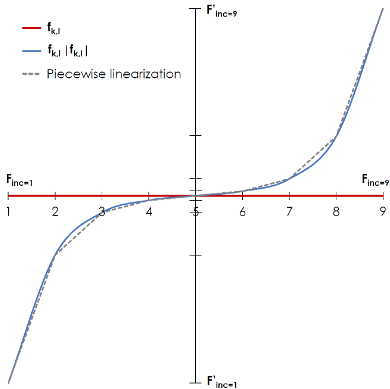
\includegraphics[width=\textwidth]{figures/Gasflow.png}
            \end{minipage}
            \hfill
            \begin{minipage}[b]{.37\textwidth}
                \begin{coloredblock}[grey]
                    \tiny
                    \textbf{Indizes}\\[.2cm]
                    \begin{tabular}{@{}p{1.5cm} l@{}}
                        $k$ & Time step \\
                        $m,n$ & Gas nodes \\
                        $l(m,n)$ & Pipeline connecting $m,n$ \\
                    \end{tabular}
                    
                    \vspace{0.5cm}
                    
                    \textbf{Variables}\\[0.2cm]
                    \begin{tabular}{@{}p{1.5cm} l@{}}
                        $f_{k,l}$ & Average gas flow \\
                        $p_{k,m}$ & Nodal gas pressure \\
                        $f_{k,l}^{in},f_{k,l}^{out}$ & In and outflowing gas \\
                        $lp_{k,l}$ & Linepack \\
                    \end{tabular}
                    
                    \vspace{0.5cm}
                    
                    \textbf{Parameter}\\[0.2cm]
                    \begin{tabular}{@{}p{1.5cm} l@{}}
                        $R_{l,G}$ & Pipeline characteristics \\
                        $LP_l$ & Linepack characteristics \\
                    \end{tabular}
                \end{coloredblock}
            \end{minipage}
        \end{column}
    \end{columns}

    \addsource{T. Klatzer, U. Bachhiesl, S. Wogrin, A. Tomasgard, „Ramping up the hydrogen sector: An energy system modeling framework“, Applied Energy 2024, doi: \href{https://doi.org/10.1016/j.apenergy.2023.122264}{10.1016/j.apenergy.2023.122264}}
\end{frame}

%% -------------------------------------------------------------------
%% Closing Slide
\section*{Closing Slide}

\begin{frame}
    \label{frame:closing_slide}
    % Insert closing slide
    \closingslide{Thank You!}{} % frametitle and subframetitle

    \addsource{Icons used in this presentation from Font Awesome (\url{https://fontawesome.com}), licensed under \href{https://creativecommons.org/licenses/by/4.0/}{CC BY 4.0}.}
\end{frame}


%% -------------------------------------------------------------------
%% Bibliography
\begin{frame}[allowframebreaks]{Bibliography}
  \printbibliography
\end{frame}

\end{document}